\section{Segmentation of land zones}
\label{sec:segmentation}

Now that all fundamentals are covered, this chapter focuses on the implementation of the neural networks. Each reference architecture from section~\ref{sec:ref_archs} will be trained and evaluated with the original hyperparameters first. Afterwards, slight modifications are applied to the architectures, to look for optimization opportunities for the task at hand.

All implementation are done in Python with the popular Keras framework backed by TensorFlow~\cite{tf_whitepaper15}. It is a well established framework with extensive tooling, lots of documentation and a great open-source community. Also it is proven to be production-ready by a broad variety of companies for all kinds of tasks\footnote{Case studies can be found at \url{https://www.tensorflow.org/about/case-studies}}. More information about tools and hardware used throughout this thesis is listed in appendix~\ref{app:tools_hardware}

\subsection{Preparing the training and test dataset}
\label{sec:prepare_train_test}
\WIP{
\cite{DLbook16}[p.~101f]
before training we have to think about how to evaluate the models afterwards. goal is to have a model that is able to generalize, meaning it should work on data that is has not seen during training. Therefore, dataset is split into two disjoint sets of data, one called the \emph{training set} and the other called \emph{test set}. During training, only data from the training set is presented to the model. afterwards, performance is measured against the test set. That way the metrics provide a more objective view on the performance.

\cite{DLbook16}[p.~119]
test set should not be used to make any choices about the model. To optimize hyperparameters for the model, another split of training data, called \emph{validation set} is introduced. Training set is used to learn parameters, validation set is used to estimate generalization error without consulting the test set. Only after hyperparameters and model weights are optimized all the way, test set is used to measure overall performance of the model.

\cite{val_split18}
There are many ways to pick data for test and validation set. An insight into common techniques is provided by \cite{val_split18}. For this thesis, test set is selected based on imbalance between categories. For each category choose $10\%$ of samples randomly and add them to test set. This is to achieve fair results taking into account all categories accordingly. Validation set also $10\%$ of training set, but chosen randomly over all samples without considering segmentation categories.

as said in \ref{sec:dataset_considerations}, big imbalance between categories in the dataset. this might lead to unwanted biases while training the model. for examples, if network predicts only forest all the time, accuracy would be around $65\%$ measured over entire dataset. plain number is not too bad, but obviously segmentation predictions would be useless.

there are some techniques to tackle those issues. one approach is to add class weights for calculating the loss function. by doing that, incorrect predictions for some classes can be punished more than others. this will result in the model being optimized in a different way, reducing the predictions for the over-represented classes. However, this was not found to work great with given dataset. all experiments had the models end up to only predict a single class for every pixel.

Another approach was selected as follows. dataset contains huge segments that all belong to same class. it was expected, that this circumstance leads to the models learning that most examples only contain one class instead of learning the differences between classes. because of that, the dataset used for training and validation was reduced by a great margin. Basically, all image files that consist of only one class for every pixel are dropped. on the one hand, this affects class imbalance, because large partitions of forests and agricultural regions are dropped, but mostly small streets and rivers are rather kept. on the other hand, this creates incentives for the models to learn the differences between classes.

% TODO: add table with category distribution of multisegment
}

\subsection{Experiments with U-Net}

\WIP{
U-Net was first architecture to explore and experiment with. Model based on findings of \cite{unet15} and explained in detail in section \ref{sec:unet}. Keras implementation used for this thesis listed in appendix~\ref{app:code}.

input image size was chosen as $572\times 572$ pixels, same as authors used. because no padding used in convolutional layers, label/prediction size is smaller, $388\times 388$ pixels for standard U-Net architecture. architecture was also evaluated with fewer/more layers, label size respectively larger/smaller.

all models trained with stochastic gradient descent optimizer with learning rate of $0.1$ and momentum of $0.99$. learning rate is reduced after every epoch to finetune model towards the end of training. Loss function was set to categorical crossentropy.

based on original model a few other configurations have been explored. base model called \texttt{U-Net-23D}. Number in the name is number of convolution layers in the model. \texttt{D} at the end if dropout layer is used for regularization. one model trained with class weights, this has \texttt{CW} at the end of name.

\ref{fig:unet_train_metrics} shows training metrics from unet models. plots are loss, categorical accuracy, mean iou per epoch calculated from validation set during training. validation data was not used for updating weights, only for evaluation. thus, the numbers provide good evidence of models generalization ability.

clearly visible that both \texttt{U-Net-23D-CW} and \texttt{U-Net-28D} did not perform well. Training was stopped after 5 epochs, because no improvement. loss for \texttt{U-Net-23D-CW} was lower than other models, this is natural, because weigts reduce the loss for some classes, but does not increase it for the others. also other metrics show that this model performed very poorly. investigation showed that \texttt{U-Net-23D-CW} only predicts forest for all pixels. \texttt{U-Net-28D} only predicts agriculture.
% TODO: validate cat. accuracy for both. 28D seems OK, but 23D-CW seems too low for forest

for \texttt{U-Net-18D} first few epochs show improvement on all metrics. level out after around 5 epochs, then only minor changes. could be that the model reached its capacity. fewer conv layers means less parameters and thus reduced ability to learn and generalize features. end up with $61\%$ categorical accuracy and $21.7\%$ mean IoU.

best results yield model with full $23$ convolution layers. with dropout, model learns a bit faster. after 20 epochs both variants arrive at around $74\%$ categorical accuracy and $42.2\%$ mean iou.

\ref{fig:unet_prediction_images} shows model predictions in test set compared to original image and ground truth. Because of U-Net architecture, label covers smaller area than original image. red border in original image indicates the area that label covers. As discussed in section \ref{sec:dataset_considerations}, labels are not super accuracy.

For \texttt{U-Net-18D} you can see that predictions ignore water. Also roads are identified as buildings instead. reduced number of parameters are not enough to make accurate predictions for those.

\texttt{U-Net-23D} and \texttt{U-Net-23} show much better results, predictions very similar to each other. first row shows that inaccurate labels are okay, model are able to abstract away the inaccurate borders. compared to original image, predictions represent riverbanks way better than ground truth.

second row shows that both models also have trouble with traffic class. both detect the road that is not described in ground truth, but label it as buildings instead of traffic.
}

\begin{figure}
    \newcommand{\UnetMetricsImageWidth}{0.32\textwidth}
    \centering
            \begin{scaletikzpicturetowidth}{\textwidth}
\begin{tikzpicture}[scale=\tikzscale]
    \begin{axis}[
        mark=x,
        cycle list name=color,
        name=unetplot1,
        xmin=1, xmax=20,
    ]

    \addplot
    coordinates{
        (1, 0.6565079689025879)
        (2, 0.6566150784492493)
        (3, 0.6565304398536682)
        (4, 0.656408965587616)
        (5, 0.6566259264945984)
    };

    \addplot
    coordinates{
        (1, 1.3805760145187378)
        (2, 1.2029350996017456)
        (3, 1.0258171558380127)
        (4, 0.9140180349349976)
        (5, 0.8663129806518555)
        (6, 0.8311066627502441)
        (7, 0.8023157715797424)
        (8, 0.8315499424934387)
        (9, 0.7800722122192383)
        (10, 0.7648837566375732)
        (11, 0.7714964747428894)
        (12, 0.7677916884422302)
        (13, 0.7400503158569336)
        (14, 0.7427014708518982)
        (15, 0.7341839075088501)
        (16, 0.7475335001945496)
        (17, 0.7335283160209656)
        (18, 0.7399769425392151)
        (19, 0.7249587774276733)
        (20, 0.732405960559845)
    };

    \addplot
    coordinates{
        (1, 1.266666054725647)
        (2, 1.2810273170471191)
        (3, 1.1684550046920776)
        (4, 1.1036863327026367)
        (5, 0.9430841207504272)
        (6, 0.904362142086029)
        (7, 0.8709024786949158)
        (8, 0.8564851880073547)
        (9, 0.8495147228240967)
        (10, 0.8020780682563782)
        (11, 0.8123838305473328)
        (12, 0.8001933693885803)
        (13, 0.7681636810302734)
        (14, 0.7739695906639099)
        (15, 0.7636772394180298)
        (16, 0.7632151246070862)
        (17, 0.7528753876686096)
        (18, 0.746317982673645)
        (19, 0.7447842955589294)
        (20, 0.7457795143127441)
    };

    \addplot
    coordinates{
        (1, 1.2214372158050537)
        (2, 1.1931297779083252)
        (3, 1.1903798580169678)
        (4, 1.1395219564437866)
        (5, 1.1235227584838867)
        (6, 1.1210097074508667)
        (7, 1.1146382093429565)
        (8, 1.1130719184875488)
        (9, 1.1082816123962402)
        (10, 1.1061081886291504)
        (11, 1.1077511310577393)
        (12, 1.1041945219039917)
        (13, 1.1035878658294678)
        (14, 1.1043835878372192)
        (15, 1.1015698909759521)
        (16, 1.1020666360855103)
        (17, 1.1022522449493408)
        (18, 1.1018295288085938)
        (19, 1.1012828350067139)
        (20, 1.0986037254333496)
    };

    \end{axis}
     \begin{axis}[
        mark=x,
        cycle list name=color,
        name=unetplot2,
        at=(unetplot1.right of south east), anchor=left of south west,
        legend style={at={(0.5,-0.25)},anchor=north},
        xmin=1, xmax=20,
    ]

    \addplot
    coordinates{
        (1, 0.33829551935195923)
        (2, 0.3379623293876648)
        (3, 0.3379237949848175)
        (4, 0.3392694592475891)
        (5, 0.33713293075561523)
    };
    \addlegendentry{U-Net-23D-CW}

    \addplot
    coordinates{
        (1, 0.33829551935195923)
        (2, 0.501347541809082)
        (3, 0.645989179611206)
        (4, 0.685759425163269)
        (5, 0.7034950852394104)
        (6, 0.7160254120826721)
        (7, 0.7236952781677246)
        (8, 0.7100507020950317)
        (9, 0.728688657283783)
        (10, 0.7320661544799805)
        (11, 0.7301645874977112)
        (12, 0.7307804226875305)
        (13, 0.7398107051849365)
        (14, 0.7392005324363708)
        (15, 0.7434249520301819)
        (16, 0.7352943420410156)
        (17, 0.7410112023353577)
        (18, 0.742379903793335)
        (19, 0.7461361289024353)
        (20, 0.744171679019928)
    };
    \addlegendentry{U-Net-23D}

    \addplot
    coordinates{
        (1, 0.5139918327331543)
        (2, 0.4997938871383667)
        (3, 0.5388210415840149)
        (4, 0.5911301374435425)
        (5, 0.6690385341644287)
        (6, 0.6867047548294067)
        (7, 0.6966053247451782)
        (8, 0.7008607387542725)
        (9, 0.7030636668205261)
        (10 0.7222729325294495)
        (11, 0.7182477712631226)
        (12, 0.719925045967102)
        (13, 0.7313004732131958)
        (14, 0.7299023866653442)
        (15, 0.7342550754547119)
        (16, 0.7329625487327576)
        (17, 0.7349392175674438)
        (18, 0.7385514378547668)
        (19, 0.7386317253112793)
        (20, 0.7358725666999817)
    };
    \addlegendentry{U-Net-23}

    \addplot
    coordinates{
        (1, 0.5371174216270447)
        (2, 0.5497292876243591)
        (3, 0.5471416711807251)
        (4, 0.5873233675956726)
        (5, 0.6028231382369995)
        (6, 0.6036145091056824)
        (7, 0.6062009930610657)
        (8, 0.6073462963104248)
        (9, 0.6079839468002319)
        (10 0.6088585257530212)
        (11, 0.60825514793396)
        (12, 0.6091040968894958)
        (13, 0.609974205493927)
        (14, 0.6084813475608826)
        (15, 0.609819769859314)
        (16, 0.6098917722702026)
        (17, 0.6100775003433228)
        (18, 0.6097120046615601)
        (19, 0.6102020740509033)
        (20, 0.6107391715049744)
    };
    \addlegendentry{U-Net-18D}

    \end{axis}

    \begin{axis}[
        mark=x,
        cycle list name=color,
        at=(unetplot2.right of south east), anchor=left of south west,
        xmin=1, xmax=20,
    ]

    \addplot
    coordinates{
        (1, 0.05638260766863823)
        (2, 0.05632704868912697)
        (3, 0.05632063373923302)
        (4, 0.056544896215200424)
        (5, 0.056188832968473434)
    };

    \addplot
    coordinates{
        (1, 0.05638260766863823)
        (2, 0.14802682399749756)
        (3, 0.26493558287620544)
        (4, 0.3173089921474457)
        (5, 0.34128832817077637)
        (6, 0.35409560799598694)
        (7, 0.3660319149494171)
        (8, 0.3550480306148529)
        (9, 0.3808368742465973)
        (10, 0.38574960827827454)
        (11, 0.38261398673057556)
        (12, 0.389729768037796)
        (13, 0.39931049942970276)
        (14, 0.3989291489124298)
        (15, 0.4041154682636261)
        (16, 0.40584757924079895)
        (17, 0.4110846519470215)
        (18, 0.4177403450012207)
        (19, 0.4257056713104248)
        (20, 0.4225998818874359)
    };

    \addplot
    coordinates{
        (1, 0.14475272595882416)
        (2, 0.13903780281543732)
        (3, 0.15666361153125763)
        (4, 0.2455795556306839)
        (5, 0.3087078332901001)
        (6, 0.3261967897415161)
        (7, 0.34233176708221436)
        (8, 0.3468801975250244)
        (9, 0.3550216257572174)
        (10, 0.37385615706443787)
        (11, 0.37024033069610596)
        (12, 0.3713560998439789)
        (13, 0.3893120288848877)
        (14, 0.3913959562778473)
        (15, 0.39039942622184753)
        (16, 0.4139955937862396)
        (17, 0.4096660614013672)
        (18, 0.41300487518310547)
        (19, 0.4125426113605499)
        (20, 0.42267632484436035)
    };

    \addplot
    coordinates{
        (1, 0.15161080658435822)
        (2, 0.1566145420074463)
        (3, 0.15519315004348755)
        (4, 0.1986483931541443)
        (5, 0.21347923576831818)
        (6, 0.2152184098958969)
        (7, 0.21574155986309052)
        (8, 0.21671517193317413)
        (9, 0.2158752679824829)
        (10, 0.21583761274814606)
        (11, 0.21597759425640106)
        (12, 0.21608270704746246)
        (13, 0.21780423820018768)
        (14, 0.21527351438999176)
        (15, 0.21591143310070038)
        (16, 0.21773125231266022)
        (17, 0.21799170970916748)
        (18, 0.21698665618896484)
        (19, 0.21827103197574615)
        (20, 0.21748535335063934)
    };

    \end{axis}

    \node[align=center] at (3.3, -0.65) {\tiny loss};
    \node[align=center] at (11, -0.65) {\tiny cat. accuracy};
    \node[align=center] at (19, -0.65) {\tiny mean IoU};
\end{tikzpicture}
\end{scaletikzpicturetowidth}

    \caption{Training metrics of different variations of U-Net}
    \label{fig:unet_train_metrics}
\end{figure}

\begin{figure}
    \newcommand{\UnetPredictionsImageWidth}{0.18\textwidth}
    \centering

    \includegraphics[width=\UnetPredictionsImageWidth]{images/unet/82607-image} \hfill
    \includegraphics[width=\UnetPredictionsImageWidth]{images/unet/82607-label} \hfill
    \includegraphics[width=\UnetPredictionsImageWidth]{images/unet/unet-18D/82607-prediction} \hfill
    \includegraphics[width=\UnetPredictionsImageWidth]{images/unet/unet-23/82607-prediction} \hfill
    \includegraphics[width=\UnetPredictionsImageWidth]{images/unet/unet-23D/82607-prediction}

    \vspace{3mm}
    \includegraphics[width=\UnetPredictionsImageWidth]{images/unet/104483-image} \hfill
    \includegraphics[width=\UnetPredictionsImageWidth]{images/unet/104483-label} \hfill
    \includegraphics[width=\UnetPredictionsImageWidth]{images/unet/unet-18D/104483-prediction} \hfill
    \includegraphics[width=\UnetPredictionsImageWidth]{images/unet/unet-23/104483-prediction} \hfill
    \includegraphics[width=\UnetPredictionsImageWidth]{images/unet/unet-23D/104483-prediction}

    \vspace{3mm}
    \includegraphics[width=\UnetPredictionsImageWidth]{images/unet/114975-image} \hfill
    \includegraphics[width=\UnetPredictionsImageWidth]{images/unet/114975-label} \hfill
    \includegraphics[width=\UnetPredictionsImageWidth]{images/unet/unet-18D/114975-prediction} \hfill
    \includegraphics[width=\UnetPredictionsImageWidth]{images/unet/unet-23/114975-prediction} \hfill
    \includegraphics[width=\UnetPredictionsImageWidth]{images/unet/unet-23D/114975-prediction}

    \vspace{3mm}
    \includegraphics[width=\UnetPredictionsImageWidth]{images/unet/138625-image} \hfill
    \includegraphics[width=\UnetPredictionsImageWidth]{images/unet/138625-label} \hfill
    \includegraphics[width=\UnetPredictionsImageWidth]{images/unet/unet-18D/138625-prediction} \hfill
    \includegraphics[width=\UnetPredictionsImageWidth]{images/unet/unet-23/138625-prediction} \hfill
    \includegraphics[width=\UnetPredictionsImageWidth]{images/unet/unet-23D/138625-prediction}

    \vspace{3mm}
    \includegraphics[width=\UnetPredictionsImageWidth]{images/unet/147352-image} \hfill
    \includegraphics[width=\UnetPredictionsImageWidth]{images/unet/147352-label} \hfill
    \includegraphics[width=\UnetPredictionsImageWidth]{images/unet/unet-18D/147352-prediction} \hfill
    \includegraphics[width=\UnetPredictionsImageWidth]{images/unet/unet-23/147352-prediction} \hfill
    \includegraphics[width=\UnetPredictionsImageWidth]{images/unet/unet-23D/147352-prediction}

    \begin{tikzpicture}
        \node[align=center] at (-1.2, 0) {\tiny Input};
        \node[align=center] at (2.0, 0) {\tiny Ground Truth};
        \node[align=center] at (5.0, 0) {\tiny U-Net-18D};
        \node[align=center] at (8.1, 0) {\tiny U-Net-23};
        \node[align=center] at (11, 0) {\tiny U-Net-23D};
    \end{tikzpicture}
    \caption{Selected predictions of different variantions of U-Net}
    \label{fig:unet_prediction_images}
\end{figure}





\subsection{Experiments with FC-DenseNet}
\WIP{
next look at results of FC-DenseNet as introduced in \ref{sec:densenet}. Also slight variations of architecture explored. also categorical crossentropy loss, but RMSProp optimizer instead of SGD. Also initial learning rate ($0.001$) lower as U-Net, as proposed by authors in \cite{denseseg17}.

Original model named \texttt{FC-DenseNet-103D} with $103$ convolution layers and dropout for regularization. Two other architectures proposed in \cite{denseseg17} with fewer convolution layers, $67$ and $56$ respectively. Also one model with compression layers before each transition down layer to condense input as in \cite{densenet18}. Compression was set to $0.5$, meaning number of feature maps is halved before transition down layer. Model has additional C in name to indicate compression.

according to metrics presented in \ref{fig:densenet_train_metrics} best model is \texttt{FC-DenseNet-103D}. Best results for all three metrics with loss of $1.17$, categorical accuracy of $62.6\%$ and mean IoU of $28.4\%$. Other variants have fewer parameters, so less capacity to learn generalization.

All models show some oscillations during middle epochs of training. Towards end of training at epoch 20, oscillation is reduced but not gone. this may come from learning rate being too high and model overshooting minimums in loss function. since learning rate is reduced after each epoch, this explains convergence towards the end.

taking into account the practical usability, it is usefull to look at actual predictions. figure \ref{fig:densenet_prediction_images} shows original image, ground truth and predictions of the models. \texttt{FC-DenseNet-103D}
 predictions are very fragmented for some regions. this indicates that confidence for predictions is rather low. other models do not show so much fragmentation.

From a visual aspect, \texttt{FC-DenseNet-103CD} and \texttt{FC-DenseNet-67D} seem to deliver best results. especially predictions for water are rather nice. However, predictions for traffic are very bad. Not a single model delivers predictions for traffic, all of them confuse it with buildings.
}

\begin{figure}
    \newcommand{\DensenetMetricsImageWidth}{0.32\textwidth}
    \centering
            \begin{subfigure}{0.32\textwidth}
\resizebox{\textwidth}{!}{\begin{tikzpicture}
    \begin{axis}[
        mark=x,
        cycle list name=mycolorlist,
        name=densenetplot1,
        xmin=1, xmax=20,
        ymin=1.0, ymax=2.5,
        xlabel={\scriptsize epoch},
        ylabel={\scriptsize loss},
        x label style={at={(axis description cs:0.5,0.05)}},
        y label style={at={(axis description cs:0.08,0.5)}},
    ]

    \addplot
    coordinates{
        (1, 1.8778098821640015)
        (2, 1.2668427228927612)
        (3, 1.2766574621200562)
        (4, 1.4314723014831543)
        (5, 1.4286470413208008)
        (6, 1.3057966232299805)
        (7, 1.2254855632781982)
        (8, 1.4993059635162354)
        (9, 1.1675904989242554)
        (10, 1.490395188331604)
        (11, 1.2040382623672485)
        (12, 1.4405009746551514)
        (13, 1.3286089897155762)
        (14, 1.210574984550476)
        (15, 1.1925950050354004)
        (16, 1.3692342042922974)
        (17, 1.2186700105667114)
        (18, 1.2532116174697876)
        (19, 1.1861357688903809)
        (20, 1.168188214302063)
    };

    \addplot
    coordinates{
        (1, 2.1999971866607666)
        (2, 1.3902311325073242)
        (3, 1.3412078619003296)
        (4, 1.2981048822402954)
        (5, 1.280882716178894)
        (6, 1.2695380449295044)
        (7, 1.3394079208374023)
        (8, 1.2355924844741821)
        (9, 1.2429777383804321)
        (10, 1.3308765888214111)
        (11, 1.2678800821304321)
        (12, 1.2725298404693604)
        (13, 1.3483526706695557)
        (14, 1.3196649551391602)
        (15, 1.2746803760528564)
        (16, 1.3376092910766602)
        (17, 1.3442707061767578)
        (18, 1.327423095703125)
        (19, 1.2989463806152344)
        (20, 1.2952357530593872)
    };

    \addplot
    coordinates{
        (1, 2.3974061012268066)
        (2, 1.3469152450561523)
        (3, 1.3552826642990112)
        (4, 1.326025128364563)
        (5, 1.3972184658050537)
        (6, 1.316970944404602)
        (7, 1.295585036277771)
        (8, 1.3838255405426025)
        (9, 1.2869324684143066)
        (10, 1.3071309328079224)
        (11, 1.3551321029663086)
        (12, 1.3308088779449463)
        (13, 1.375392198562622)
        (14, 1.34626042842865)
        (15, 1.3224772214889526)
        (16, 1.3284034729003906)
        (17, 1.3779839277267456)
        (18, 1.3398308753967285)
        (19, 1.3465551137924194)
        (20, 1.3300797939300537)
    };

    \addplot
    coordinates{
        (1, 1.990792155265808)
        (2, 1.294736623764038)
        (3, 1.2612152099609375)
        (4, 1.2450172901153564)
        (5, 1.24184250831604)
        (6, 1.2792901992797852)
        (7, 1.2662909030914307)
        (8, 1.37437903881073)
        (9, 1.2648396492004395)
        (10, 1.2657694816589355)
        (11, 1.316687822341919)
        (12, 1.4254909753799438)
        (13, 1.2919646501541138)
        (14, 1.3055157661437988)
        (15, 1.285273790359497)
        (16, 1.3169896602630615)
        (17, 1.3447442054748535)
        (18, 1.303223967552185)
        (19, 1.2977485656738281)
        (20, 1.2806230783462524)
    };

    \end{axis}
\end{tikzpicture}}
    \caption{}
    \label{fig:metrics_densenet_loss}
\end{subfigure}
\begin{subfigure}{0.32\textwidth}
\resizebox{\textwidth}{!}{\begin{tikzpicture}
     \begin{axis}[
        mark=x,
        cycle list name=mycolorlist,
        name=densenetplot2,
        at=(densenetplot1.right of south east), anchor=left of south west,
        legend style={at={(0.77,0.32)},anchor=north},
        xmin=1, xmax=20,
        ymin=0.2, ymax=0.7,
        xlabel={\scriptsize epoch},
        ylabel={\scriptsize loss},
        x label style={at={(axis description cs:0.5,0.05)}},
        y label style={at={(axis description cs:0.08,0.5)}},
    ]

    \addplot
    coordinates{
        (1, 0.44403234124183655)
        (2, 0.5382390022277832)
        (3, 0.5460906624794006)
        (4, 0.5117834806442261)
        (5, 0.49210643768310547)
        (6, 0.5355142951011658)
        (7, 0.5704494714736938)
        (8, 0.4416641891002655)
        (9, 0.6110737323760986)
        (10, 0.4632301926612854)
        (11, 0.590806782245636)
        (12, 0.5226526260375977)
        (13, 0.5564858317375183)
        (14, 0.5993890166282654)
        (15, 0.613778829574585)
        (16, 0.5397917628288269)
        (17, 0.5880735516548157)
        (18, 0.5896559357643127)
        (19, 0.6149882078170776)
        (20, 0.6262763142585754)
    };
    \addlegendentry{\scriptsize FCDN-103D}

    \addplot
    coordinates{
        (1, 0.31083741784095764)
        (2, 0.4629298746585846)
        (3, 0.47024381160736084)
        (4, 0.5197407603263855)
        (5, 0.5138208270072937)
        (6, 0.5358591675758362)
        (7, 0.4863249957561493)
        (8, 0.5566446781158447)
        (9, 0.5620558261871338)
        (10, 0.49684542417526245)
        (11, 0.5612539649009705)
        (12, 0.5544501543045044)
        (13, 0.5163871049880981)
        (14, 0.5430474281311035)
        (15, 0.5622951984405518)
        (16, 0.5312788486480713)
        (17, 0.5277349352836609)
        (18, 0.5413538217544556)
        (19, 0.5542507767677307)
        (20, 0.5590786933898926)
    };
    \addlegendentry{\scriptsize FCDN-103CD}

    \addplot
    coordinates{
        (1, 0.24311639368534088)
        (2, 0.4761204421520233)
        (3, 0.4544506072998047)
        (4, 0.4913800060749054)
        (5, 0.41295066475868225)
        (6, 0.5058783292770386)
        (7, 0.5192673206329346)
        (8, 0.4526740610599518)
        (9, 0.5332894325256348)
        (10, 0.5307732820510864)
        (11, 0.5094674229621887)
        (12, 0.5299655795097351)
        (13, 0.49733099341392517)
        (14, 0.5140370726585388)
        (15, 0.5340467691421509)
        (16, 0.525802493095398)
        (17, 0.499888151884079)
        (18, 0.5290431976318359)
        (19, 0.5265495777130127)
        (20, 0.5373263955116272)
    };
    \addlegendentry{\scriptsize FCDN-67D}

    \addplot
    coordinates{
        (1, 0.3250448405742645)
        (2, 0.5240246057510376)
        (3, 0.5330521464347839)
        (4, 0.5476676821708679)
        (5, 0.5379430651664734)
        (6, 0.5243373513221741)
        (7, 0.5286471247673035)
        (8, 0.47282737493515015)
        (9, 0.5424470901489258)
        (10, 0.5523974299430847)
        (11, 0.5108893513679504)
        (12, 0.5004795789718628)
        (13, 0.5263856053352356)
        (14, 0.5332449078559875)
        (15, 0.5562388896942139)
        (16, 0.534349262714386)
        (17, 0.5274752974510193)
        (18, 0.5481530427932739)
        (19, 0.5545112490653992)
        (20, 0.5611099600791931)
    };
    \addlegendentry{\scriptsize FCDN-56D}

    \end{axis}
\end{tikzpicture}}
    \caption{}
    \label{fig:metrics_densenet_catacc}
\end{subfigure}
\begin{subfigure}{0.32\textwidth}
\resizebox{\textwidth}{!}{\begin{tikzpicture}
    \begin{axis}[
        mark=x,
        cycle list name=mycolorlist,
        at=(densenetplot2.right of south east), anchor=left of south west,
        xmin=1, xmax=20,
        ymin=0, ymax=0.35,
        ymin=0.0, ymax=0.35,
        xlabel={\scriptsize epoch},
        ylabel={\scriptsize loss},
        x label style={at={(axis description cs:0.5,0.05)}},
        y label style={at={(axis description cs:0.08,0.5)}},
    ]

    \addplot
    coordinates{
        (1, 0.15961624681949615)
        (2, 0.23034006357192993)
        (3, 0.2510993778705597)
        (4, 0.2040325254201889)
        (5, 0.15874336659908295)
        (6, 0.2393379658460617)
        (7, 0.2576610743999481)
        (8, 0.20172123610973358)
        (9, 0.28852298855781555)
        (10, 0.1903650313615799)
        (11, 0.2816150486469269)
        (12, 0.2380661964416504)
        (13, 0.2526349425315857)
        (14, 0.28796717524528503)
        (15, 0.29596516489982605)
        (16, 0.2512836754322052)
        (17, 0.2903881371021271)
        (18, 0.28366556763648987)
        (19, 0.30205875635147095)
        (20, 0.28375494480133057)
    };

    \addplot
    coordinates{
        (1, 0.08612015843391418)
        (2, 0.18902510404586792)
        (3, 0.18584029376506805)
        (4, 0.2238929122686386)
        (5, 0.21692800521850586)
        (6, 0.2446306347846985)
        (7, 0.19728021323680878)
        (8, 0.254301518201828)
        (9, 0.2588264048099518)
        (10, 0.21687805652618408)
        (11, 0.2554681599140167)
        (12, 0.24556516110897064)
        (13, 0.21257217228412628)
        (14, 0.23620039224624634)
        (15, 0.23790551722049713)
        (16, 0.2152477353811264)
        (17, 0.2248375415802002)
        (18, 0.2260301262140274)
        (19, 0.2301390916109085)
        (20, 0.240129753947258)
    };

    \addplot
    coordinates{
        (1, 0.05528780445456505)
        (2, 0.2058449238538742)
        (3, 0.1926068663597107)
        (4, 0.1960599273443222)
        (5, 0.1480538696050644)
        (6, 0.21407771110534668)
        (7, 0.22343073785305023)
        (8, 0.1498967856168747)
        (9, 0.21587294340133667)
        (10, 0.23544591665267944)
        (11, 0.21624718606472015)
        (12, 0.21524637937545776)
        (13, 0.1991012543439865)
        (14, 0.2097732275724411)
        (15, 0.2226145714521408)
        (16, 0.21674305200576782)
        (17, 0.21302568912506104)
        (18, 0.21026158332824707)
        (19, 0.22532594203948975)
        (20, 0.23161913454532623)
    };

    \addplot
    coordinates{
        (1, 0.13292203843593597)
        (2, 0.22567109763622284)
        (3, 0.23399783670902252)
        (4, 0.2489478588104248)
        (5, 0.19032984972000122)
        (6, 0.2309076339006424)
        (7, 0.2147936075925827)
        (8, 0.1856151819229126)
        (9, 0.20955342054367065)
        (10, 0.24931295216083527)
        (11, 0.20019109547138214)
        (12, 0.17687444388866425)
        (13, 0.18552462756633759)
        (14, 0.19671611487865448)
        (15, 0.21579863131046295)
        (16, 0.1941973716020584)
        (17, 0.21591031551361084)
        (18, 0.20780526101589203)
        (19, 0.2145579308271408)
        (20, 0.21770614385604858)
    };

    \end{axis}
\end{tikzpicture}}
    \caption{}
    \label{fig:metrics_densenet_iou}
\end{subfigure}

    \caption{Training metrics of different variations of FC-DenseNet}
    \label{fig:densenet_train_metrics}
\end{figure}

\begin{figure}
    \newcommand{\DensenetPredictionsImageWidth}{0.15\textwidth}
    \centering

    \includegraphics[width=\DensenetPredictionsImageWidth]{images/densenet/101444-image} \hfill
    \includegraphics[width=\DensenetPredictionsImageWidth]{images/densenet/101444-label} \hfill
    \includegraphics[width=\DensenetPredictionsImageWidth]{images/densenet/densenet-103D/101444-prediction} \hfill
    \includegraphics[width=\DensenetPredictionsImageWidth]{images/densenet/densenet-103CD/101444-prediction} \hfill
    \includegraphics[width=\DensenetPredictionsImageWidth]{images/densenet/densenet-67D/101444-prediction} \hfill
    \includegraphics[width=\DensenetPredictionsImageWidth]{images/densenet/densenet-56D/101444-prediction}

    \vspace{3mm}
    \includegraphics[width=\DensenetPredictionsImageWidth]{images/densenet/291991-image} \hfill
    \includegraphics[width=\DensenetPredictionsImageWidth]{images/densenet/291991-label} \hfill
    \includegraphics[width=\DensenetPredictionsImageWidth]{images/densenet/densenet-103D/291991-prediction} \hfill
    \includegraphics[width=\DensenetPredictionsImageWidth]{images/densenet/densenet-103CD/291991-prediction} \hfill
    \includegraphics[width=\DensenetPredictionsImageWidth]{images/densenet/densenet-67D/291991-prediction} \hfill
    \includegraphics[width=\DensenetPredictionsImageWidth]{images/densenet/densenet-56D/291991-prediction}

    \vspace{3mm}
    \includegraphics[width=\DensenetPredictionsImageWidth]{images/densenet/436897-image} \hfill
    \includegraphics[width=\DensenetPredictionsImageWidth]{images/densenet/436897-label} \hfill
    \includegraphics[width=\DensenetPredictionsImageWidth]{images/densenet/densenet-103D/436897-prediction} \hfill
    \includegraphics[width=\DensenetPredictionsImageWidth]{images/densenet/densenet-103CD/436897-prediction} \hfill
    \includegraphics[width=\DensenetPredictionsImageWidth]{images/densenet/densenet-67D/436897-prediction} \hfill
    \includegraphics[width=\DensenetPredictionsImageWidth]{images/densenet/densenet-56D/436897-prediction}

    \vspace{3mm}
    \includegraphics[width=\DensenetPredictionsImageWidth]{images/densenet/626312-image} \hfill
    \includegraphics[width=\DensenetPredictionsImageWidth]{images/densenet/626312-label} \hfill
    \includegraphics[width=\DensenetPredictionsImageWidth]{images/densenet/densenet-103D/626312-prediction} \hfill
    \includegraphics[width=\DensenetPredictionsImageWidth]{images/densenet/densenet-103CD/626312-prediction} \hfill
    \includegraphics[width=\DensenetPredictionsImageWidth]{images/densenet/densenet-67D/626312-prediction} \hfill
    \includegraphics[width=\DensenetPredictionsImageWidth]{images/densenet/densenet-56D/626312-prediction}

    \vspace{3mm}
    \includegraphics[width=\DensenetPredictionsImageWidth]{images/densenet/768909-image} \hfill
    \includegraphics[width=\DensenetPredictionsImageWidth]{images/densenet/768909-label} \hfill
    \includegraphics[width=\DensenetPredictionsImageWidth]{images/densenet/densenet-103D/768909-prediction} \hfill
    \includegraphics[width=\DensenetPredictionsImageWidth]{images/densenet/densenet-103CD/768909-prediction} \hfill
    \includegraphics[width=\DensenetPredictionsImageWidth]{images/densenet/densenet-67D/768909-prediction} \hfill
    \includegraphics[width=\DensenetPredictionsImageWidth]{images/densenet/densenet-56D/768909-prediction}

    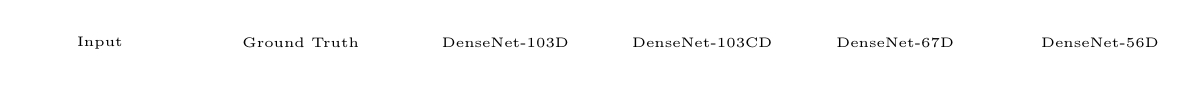
\begin{tikzpicture}
        \node[align=center] at (0, 0) {};
        \node[align=center] at (0.8, 0) {\tiny Input};
        \node[align=center] at (3.35, 0) {\tiny Ground Truth};
        \node[align=center] at (5.95, 0) {\tiny DenseNet-103D};
        \node[align=center] at (8.45, 0) {\tiny DenseNet-103CD};
        \node[align=center] at (10.9, 0) {\tiny DenseNet-67D};
        \node[align=center] at (13.5, 0) {\tiny DenseNet-56D};
    \end{tikzpicture}
    \caption{Selected predictions of different variantions of FC-DenseNet}
    \label{fig:densenet_prediction_images}
\end{figure}

\subsection{Experiments with W-Net}
\WIP{
\begin{itemize}
    \item show the architectures of all W-Net models
    \item describe the idea behind the architectural decisions
\end{itemize}
}

\subsection{Discussion}
\WIP{
\begin{itemize}
    \item have a look at the segments that were found by the NN
    \item show segmentation results of large areas
    \item compare segments to the real landscape in the dataset
    \item discuss practical use of those results for identifying emergency landing fields
    \item evaluate results and assess which data to use for the vegetation analysis
\end{itemize}
}

\newpage
